\subsection{Approximating the Step Response}

So far, two methods for characterising step response functions were illustrated,
namely the method proposed  by  P.  Hudzovic (equation \ref{eq:tu_tg}) where you
calculate  $T_u$  and  $T_g$,  and  the  method  proposed by L.  Sani  (equation
\ref{eq:t10_t50_t90})   where  you  calculate  $t_{10}$,   $t_{50}$,   $t_{90}$.

Furthermore, two similar methods for constructing a transfer function $G_n(s,r)$
(equation \ref{eq:ptn}) were shown, again, one proposed by P. Hudzovic (equation
\ref{eq:hudzovic})  and  one  proposed by L. Sani (equation  \ref{eq:sani})  for
calculating the individual time constants $T_1 \ldots T_n$ based  on  the  input
parameters $r$ and $T$.

By  combining  the  various  approaches  with each other, 4 different  ways  for
determining $G_n(s,r)$ exist.

It  is  not  possible to \textit{directly} calculate appropriate values for $n$,
$T$  and $r$ when given an unknown step response  function,  however,  by  using
equations \ref{eq:ptn},  \ref{eq:hudzovic}  and \ref{eq:sani}, it is possible to
construct  a  lookup table by calculating a (theoretically) infinite  number  of
step responses in function of $n$  and  $r$,  characterise  their  step response
using  equations \ref{eq:tu_tg} or \ref{eq:t10_t50_t90}  (i.e.  determine  their
``complexity''), and perform a  reverse  lookup  on  those  results  to find the
parameters $n$, $r$.  This method of reverse lookup works because -- as you will
soon  see  --  the   lookup   curves  are  monotonically  increasing/decreasing.

In practice, it  is  sufficient  to  calculate  about 50 step responses for each
order  $n$  and  interpolate  between  those values when performing the  lookup.

As mentioned earlier, a remarkable  observation  is  that the parameters $r$ and
$n$ are independent of time and amplitude (and offset); that is,  the normalised
step response does not change its  shape when the parameter $T$ is changed. This
is fantastic,  because  it  allows  us  to eliminate a dimension from the lookup
table.

If $T=1$, $K_s=1$  and  $y_0=0$,  equations  \ref{eq:ptn}, \ref{eq:hudzovic} and
\ref{eq:sani}  can  be   used  to  calculate  a  series  of  transfer  functions
$G_n(s,r)$, their time domain step responses $g_{r,n}(t)$ can be calculated, and
they  can  be  characterised  by  calculating $g_{T_u/T_g}$  and  $g_{\lambda}$.

These two values alone aren't yet enough. The  result will still be dependent on
$T_g$ or $t_{50}$. In order to fully ``denormalise'' the result, $g_{1/T_g}$ and
$g_{1/t_{50}}$ must also be calculated for each step response.

\clearpage

\begin{figure}[t]
    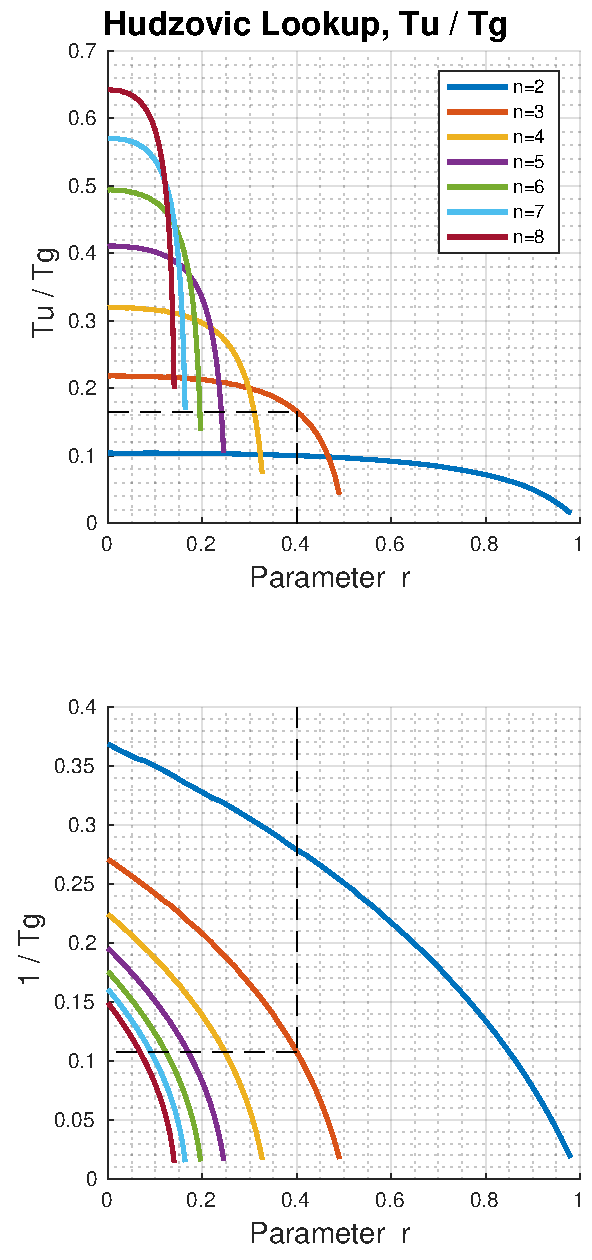
\includegraphics[width=\linewidth]{images/hudzovic_curves_tu_tg}
    \caption{P. Hudzovic lookup curves. Top: Tu/Tg, bottom:1/Tg}
    \label{fig:hudzovic_tu_tg}
\end{figure}
\begin{figure}[t]
    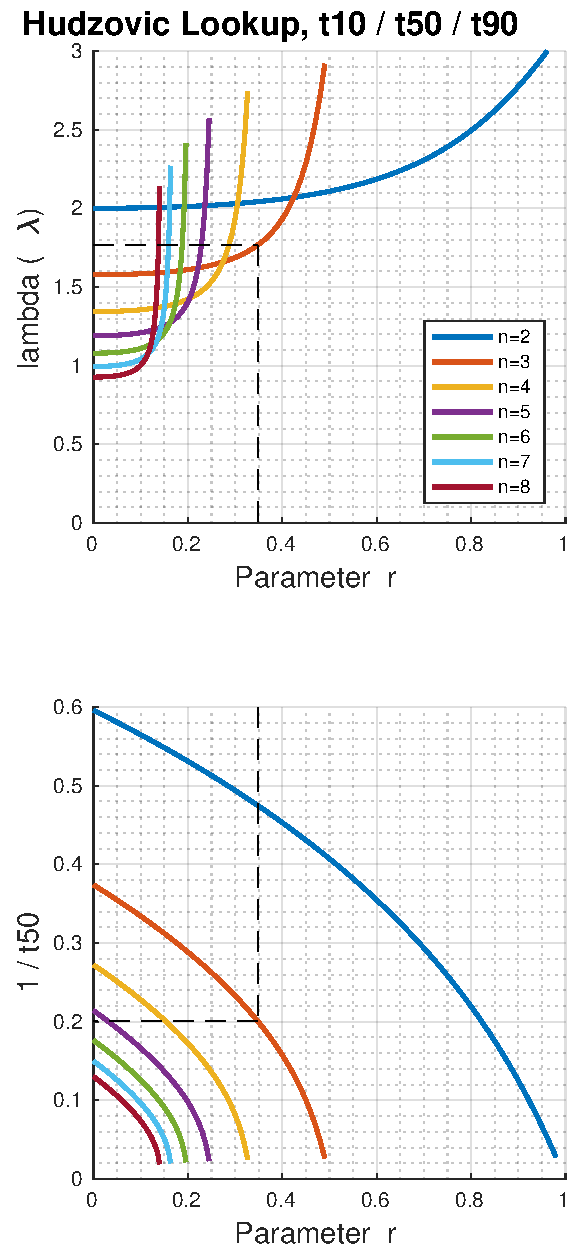
\includegraphics[width=\linewidth]{images/hudzovic_curves_t10_t50_t90}
    \caption{P. Hudzovic lookup curves. Top: (t90-t10/t50), bottom: 1/t50}
    \label{fig:hudzovic_t3}
\end{figure}

\clearpage

\begin{figure}[t]
    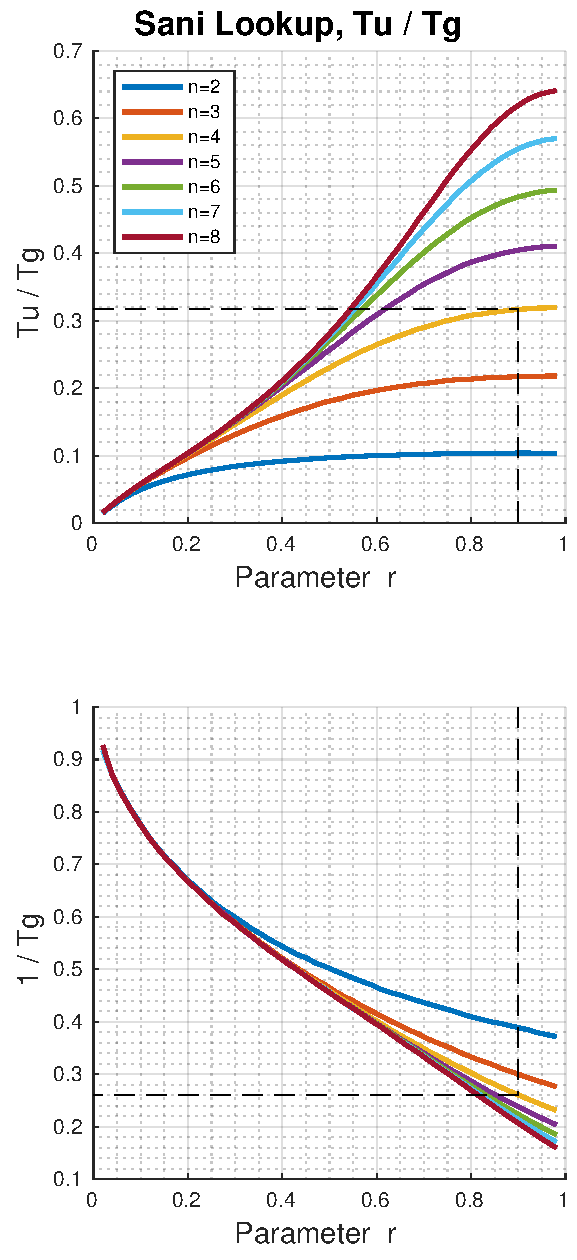
\includegraphics[width=\linewidth]{images/sani_curves_tu_tg}
    \caption{L. Sani lookup curves. Top: Tu/Tg, bottom: 1/Tg lookup}
    \label{fig:sani_tu_tg}
\end{figure}
\begin{figure}[t]
    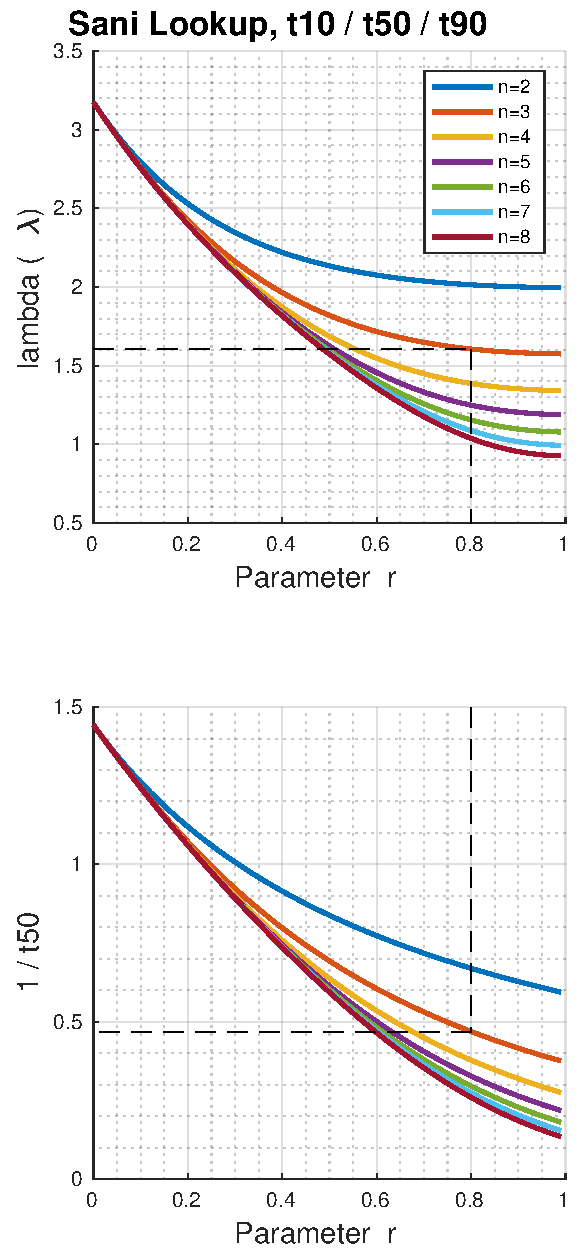
\includegraphics[width=\linewidth]{images/sani_curves_t10_t50_t90}
    \caption{L. Sani lookup curves. Top: (t90-t10)/t50, bottom: 1/t50}
    \label{fig:sani_t3}
\end{figure}

\clearpage

The various characterisations of the step response  function  $g(t)$  can all be
expressed as functions of $r$ and $n$:

\begin{align}
    g_{T_u/T_g}  &= g_{T_u/T_g}(r, n) \\
    g_{1/T_g}    &= g_{1/T_g}(r,n) \\
    g_{\lambda}  &= g_{\lambda}(r,n) \\
    g_{1/t_{50}} &= g_{1/t_{50}}(r,n)
\end{align}

Using P.  Hudzovic's  approach from equations \ref{eq:ptn} and \ref{eq:hudzovic}
the four functions $g_{T_u/T_g}(r, n)$, $g_{1/T_g}(r,n)$, $g_{\lambda}(r,n)$ and
$g_{1/t_{50}}(r,n)$  are  evaluated.  The figures  \ref{fig:hudzovic_tu_tg}  and
\ref{fig:hudzovic_t3} are obtained.

Similarly,  using   L.   Sani's   approach   from   equations  \ref{eq:ptn}  and
\ref{eq:sani} we  again  evaluate the same four functions and obtain the figures
\ref{fig:sani_tu_tg} and \ref{fig:sani_t3}.

What these plots show beautifully is that the  higher the order $n$, the steeper
-- or more ``complex'' -- the step response becomes (smaller  values of $T_g$ or
$t_{90}-t_{10}$ mean faster rise times of the step responses). Another important
thing  to observe is how lower orders of $G_n(s,r)$ aren't able to rise as  fast
as higher orders are able to, \textbf{regardless} of $r$ and $T$.  This can also
be seen in all four figures: Lower orders  cannot  reach  ratios of $T_u/T_g$ or
$\lambda$ that higher orders can.


\subsubsection*{Calculating T, r, n, by using Lookup Curves}

As already mentioned, determining the  complexity of a step response is directly
related  to  the  required  order $n$ of the model. Finding $n$ is now a  simple
matter of computing $\textrm{plant}_{T_u/T_g}$ or $\textrm{plant}_{\lambda}$ and
iterating     through    the    different    curves     either     in     figure
\ref{fig:hudzovic_tu_tg},   \ref{fig:sani_tu_tg},    \ref{fig:hudzovic_t3},   or
\ref{fig:sani_t3}  until  a value of $n$ is found that satisfies one  of  either
conditions:

\begin{align}
    g_{T_u/T_g}(r, n)\lvert_{r=max} \hspace{2mm} &\le \hspace{2mm} plant_{T_u/T_g} \\
    g_{\lambda}(r, n)\lvert_{r=max} \hspace{2mm} &\le \hspace{2mm} plant_{\lambda} \label{eq:find_n}
\end{align}

Ideally, $n$ should be as small as possible.

With the parameter $n$ defined, the next step is to find the  intersection point
of the horizontal line that passes through either  $\textrm{plant}_{T_u/T_g}$ or
$\textrm{plant}_{\lambda}$   and   $g_{T_u/T_g}(r,n)$   or   $g_{\lambda}(r,n)$,
respectively.  This will yield parameter $r$. This can be achieved by solving  a
simple  line  intersection  equation  and plugging in the locations of  the  two
horizontal lines.

The   last   parameter,   $T$,   can  finally  be   determined   by   evaluating
$\textrm{plant}_{g_{1/T_g}}(r,    n)$    or    $\textrm{plant}_{t_{50}}    \cdot
g_{1/t_{50}}$ Graphically, this equates to finding the intersection point of the
vertical line going through $r$ and the function  $g_{1/T_g}(r,  n)$  in  figure
\ref{fig:hudzovic_tu_tg} and multiplying the result by $T_g$.

Each    of   the   figures    \ref{fig:hudzovic_tu_tg},    \ref{fig:sani_tu_tg},
\ref{fig:hudzovic_t3}, and \ref{fig:sani_t3}  contain  a  dashed  line, which is
supposed to demonstrate  an  example  lookup,  to  help  visualise  the process.


\subsubsection*{Calculating T, r, n, by using Interpolation Formulae}

Instead   of   having   to   generate  the  lookup   curves   seen   in   figure
\ref{fig:sani_t3},  Sani\cite{ref:sani} included two formulae that very  closely
approximate these curves. They are:

\begin{equation}
    \frac{t_{50}}{T} = \log(2)-1+\frac{1-r^{n}}{1-r}
    \label{eq:T_t50}
\end{equation}
\begin{equation}
    \frac{t_{90}-t_{10}}{T} = 1.315 \sqrt{3.8\frac{1-r^{2n}}{1-r^2} - 1}
\end{equation}

Using  the  formula for calculating $\lambda$ in equation  \ref{eq:t10_t50_t90},
the interpolation formulae can be made independent of $T$:

\begin{equation}
    \frac{t_{90}-t_{10}}{t_{50}} = \frac{1.315 \sqrt{3.8\frac{1-r^{2n}}{1-r^2} - 1}}{\log(2)-1+\frac{1-r^{n}}{1-r}}
    \label{eq:sani_interpolation}
\end{equation}

Plotting  the  functions $\frac{t_{90}-t_{10}}{t_{50}}$  and  $\frac{1}{t_{50}}$
yields  nearly  identical   curves   as   seen   in   figure  \ref{fig:sani_t3}.

The benefit of using these interpolation formulae over a lookup table is ease of
implementation, lower memory footprint and  flexibility.  Orders  of  $n$ can be
chosen  arbitrarily,  whereas  with lookup tables an entry must exist for  every
order that should be supported.

Finding the parameter $n$ is identical to the previous  example  using  equation
\ref{eq:find_n}, except that instead of  using  a  lookup table, the function in
equation \ref{eq:sani_interpolation} is evaluated.

Finding the parameter $r$ can be achieved by performing a binary search  on  the
function  in  equation  \ref{eq:sani_interpolation}.  This   works  because  the
function is monotonically decreasing.

Finding $T$ is  a  simple  matter  of  solving  equation  \ref{eq:T_t50} for the
parameter $T$ and  evaluating  it using the found parameters $n$, $r$ as well as
the plant's $t_{50}$ value $\textrm{plant}_{t_{50}}$.

